% Provenance (never printed): cycle 4 SVT, "La planete Terre": sedimentation,
% from sediment to sedimentary rock, fossilisation, fossils and layers as a
% record of past environments; see sources/book1/PROVENANCE.md. Book 1,
% grade 7, chapter 4.
% Vocabulary guard: first chapter allowed to use "sediment"; the principles of
% relative dating (superposition, fossil succession and the rest) and "unconformity" are
% g7.5's and are not named here; fossils as evidence of evolution are the
% biology books' (one sentence of prose).
\chapter{Sediments and Fossils}\label{ch:g7:sediments-and-fossils}

The Grand Canyon, in Arizona (United States), is on average
\qty{1.6}{km} deep. Its walls are made of layers of \omterm{def:g3:stones-pebbles-sand:rock}{rock}, one on top of
the other, red, brown, grey and cream. In the topmost layer, the Kaibab
Limestone, the rangers point out shells: the shells of brachiopods,
animals that lived on the floor of a \omterm{def:g2:water-on-earth:ocean}{sea}. That \omterm{def:g3:stones-pebbles-sand:rock}{rock} formed at the bottom
of an \omterm{def:g2:water-on-earth:ocean}{ocean}, and it now forms the rim of the canyon, high above the \omterm{def:g2:water-on-earth:ocean}{sea}.
% ledger: nps:grca-depth, nps:grca-fossils, nps:grca-kaibab

\begin{omfigure}
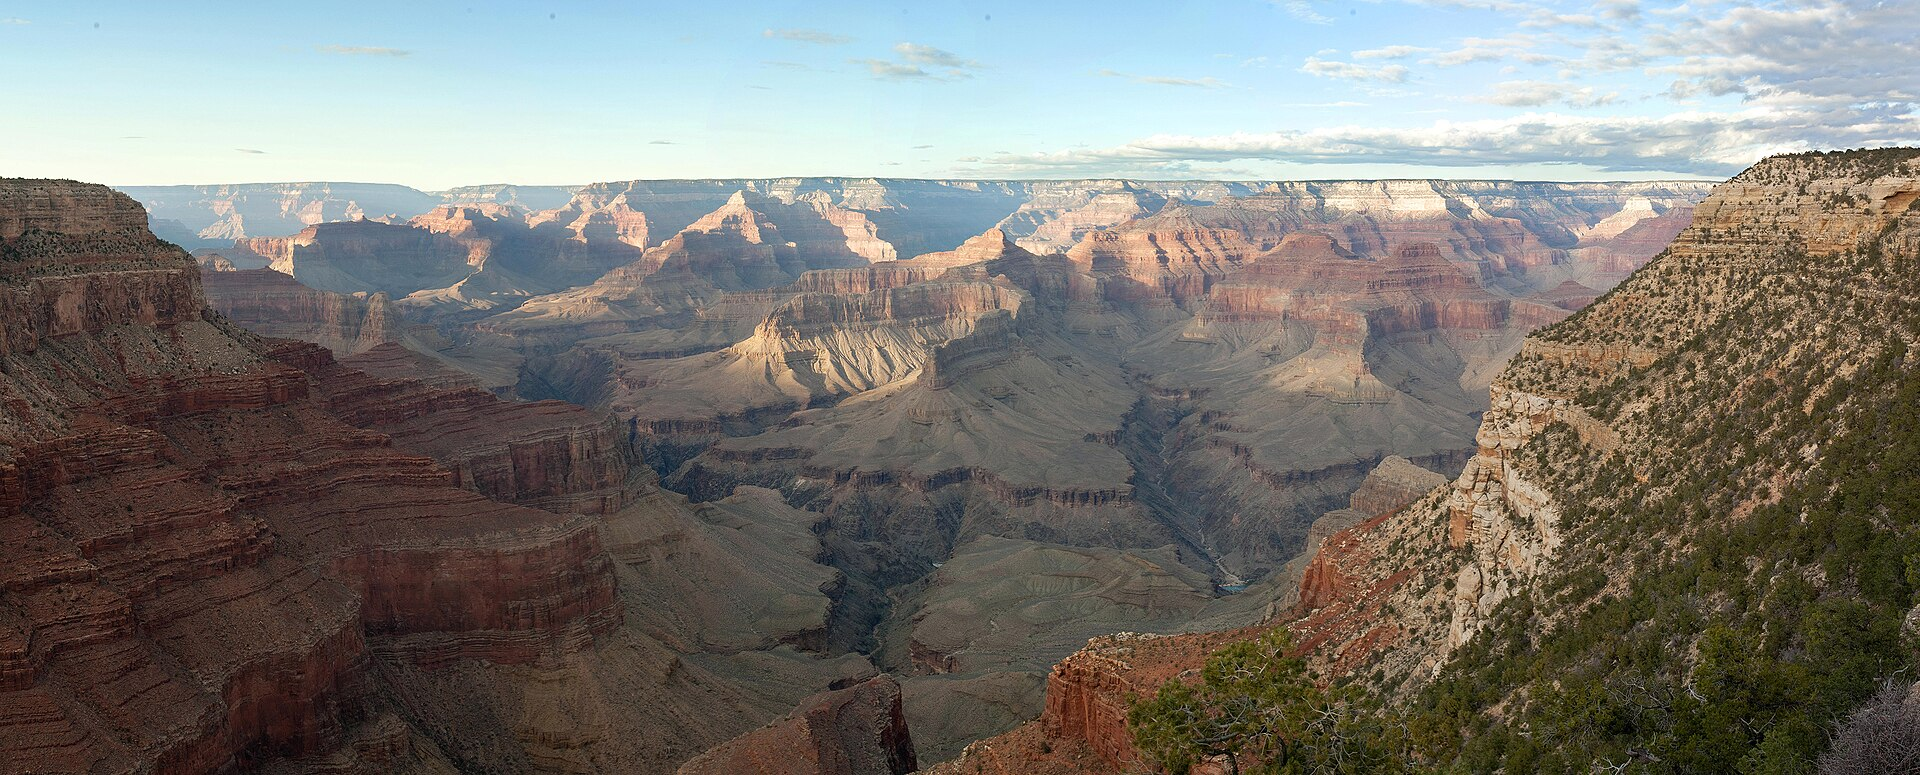
\includegraphics[width=\linewidth]{images/book1/g7-grand-canyon.jpg}

{\small The Grand Canyon from Hermits Rest, on its southern rim: layer
after layer of \omterm{def:g3:stones-pebbles-sand:rock}{rock}, from the rim down to the bottom. NPS photograph by
Kristen M. Caldon (public domain, via Wikimedia Commons).}
% ledger: commons:grand-canyon
\label{fig:g7:sediments-and-fossils:canyon}
\end{omfigure}

How does a pile of loose \omterm{def:g3:stones-pebbles-sand:sand}{sand} and \omterm{def:g3:stones-pebbles-sand:sand}{mud} become solid \omterm{def:g3:stones-pebbles-sand:rock}{rock}? How can a shell
last for so long that it ends up inside a cliff? And what do layers and
\omterm{def:g7:sediments-and-fossils:fossil}{fossils} tell us about places as they were long ago?

\begin{recall}
\omterm{def:g3:stones-pebbles-sand:rock}{Rocks} are slowly broken into pieces at the surface (\emph{\omterm{def:g5:water-shapes-the-land:weathering}{weathering}});
water, wind and ice carry the pieces away (\emph{\omterm{def:g5:water-shapes-the-land:erosion}{erosion}}) and lay them
down where they slow down and stop (\emph{\omterm{def:g5:water-shapes-the-land:deposition}{deposition}}): the heaviest
first, the fine \omterm{def:g3:stones-pebbles-sand:sand}{mud} only where the water is almost still
(\cref{ch:g5:water-shapes-the-land}). A \emph{\omterm{def:g6:rocks-and-minerals:rock-families}{sedimentary rock}} forms at
the surface from grains of \omterm{def:g3:stones-pebbles-sand:sand}{sand} and \omterm{def:g3:stones-pebbles-sand:sand}{mud}, or from shells, laid down in
layers and hardened: sandstone, shale, limestone. The \omterm{def:g6:rocks-and-minerals:rock-cycle}{rock cycle} turns
the \omterm{def:g3:stones-pebbles-sand:rock}{rocks} of each family, slowly, into the others
(\cref{ch:g6:rocks-and-minerals}).
\end{recall}

\section{Sediments settle in layers}

Wherever water, wind or ice drops what it was carrying, a loose deposit
builds up: \omterm{def:g3:stones-pebbles-sand:pebble}{gravel} and \omterm{def:g3:stones-pebbles-sand:sand}{sand} on a \omterm{def:g1:landscapes-around-us:water}{river} bed, \omterm{def:g3:stones-pebbles-sand:sand}{mud} on the bottom of a \omterm{def:g1:landscapes-around-us:water}{lake},
\omterm{def:g3:stones-pebbles-sand:sand}{sand} on a beach or in a dune, shells on the floor of the \omterm{def:g2:water-on-earth:ocean}{sea}.

\begin{definition}[Sediment]\label{def:g7:sediments-and-fossils:sediment}
A \emph{sediment}\index{sediment} is loose material laid down by water,
wind or ice: \omterm{def:g3:stones-pebbles-sand:pebble}{gravel}, \omterm{def:g3:stones-pebbles-sand:sand}{sand}, \omterm{def:g3:stones-pebbles-sand:sand}{mud}, or the shells and skeletons of living
things. It collects at the bottom of \omterm{def:g1:landscapes-around-us:water}{rivers}, \omterm{def:g1:landscapes-around-us:water}{lakes} and \omterm{def:g2:water-on-earth:ocean}{seas}, and on land
where the wind or the ice drops it.
\end{definition}

\omterm{def:g7:sediments-and-fossils:sediment}{Sediments} settle in a particular order. When muddy water slows down, the
largest and heaviest grains sink first and the smallest and lightest
last. Each time the water changes --- a \omterm{def:g5:water-shapes-the-land:flood}{flood} that brings \omterm{def:g3:stones-pebbles-sand:sand}{sand}, then calm
weeks when only fine \omterm{def:g3:stones-pebbles-sand:sand}{mud} reaches the bottom --- the grains that settle
change too, and a new layer starts. Little by little, the bottom of a
\omterm{def:g1:landscapes-around-us:water}{lake} or of a \omterm{def:g2:water-on-earth:ocean}{sea} is covered with a pile of layers, the oldest at the
bottom of the pile.
% ledger: usgs:strata, usgs:sediments-to-rock

\begin{omfigure}
\begin{tikzpicture}[font=\small, x=1cm, y=1cm]
  % land and river
  \fill[omLithAlluv] (0,3.0) -- (2.0,2.45) -- (2.0,0) -- (0,0) -- cycle;
  \fill[blue!35] (0,3.05) -- (2.0,2.5) -- (2.0,2.4) -- (0,2.95) -- cycle;
  % lake water
  \fill[omSea!45] (2.0,2.5) -- (12.4,2.5) -- (12.4,1.12) -- (3.0,1.2) -- cycle;
  \draw[blue!50!black, line width=0.6pt] (2.0,2.5) -- (12.4,2.5);
  % layers on the bottom: thick near the mouth, thinner far out
  \foreach \k/\c in {0/omLithSand, 1/omLithShale, 2/omLithSand, 3/omLithShale} {
    \pgfmathsetmacro{\yb}{0.2+0.25*\k}
    \pgfmathsetmacro{\yt}{0.2+0.25*(\k+1)}
    \fill[\c] (3.0,\yb) -- (12.4,\yb) -- (12.4,\yt-0.08) -- (3.0,\yt) -- cycle;
  }
  \draw[black!60, line width=0.3pt] (3.0,1.2) -- (12.4,1.12);
  \fill[omLithAlluv!80!black] (2.0,0) rectangle (12.4,0.2);
  \fill[omLithAlluv] (2.0,0.2) -- (3.0,0.2) -- (3.0,1.2) -- (2.0,2.45) -- cycle;
  % settling grains: big ones near the mouth, fine ones far out
  \foreach \x/\y in {3.3/2.1, 3.6/1.75, 3.9/2.25, 4.2/1.55, 3.5/1.35, 4.5/2.0} {
    \fill[brown!70!black] (\x,\y) circle (0.07);
    \draw[-{Stealth[length=1.3mm]}, black!60] (\x,\y-0.1) -- (\x,\y-0.32);
  }
  \foreach \x/\y in {6.5/2.2, 7.4/1.8, 8.3/2.15, 9.1/1.6, 9.9/2.05, 10.8/1.75, 11.6/2.1, 7.9/1.35, 10.4/1.3} {
    \fill[brown!50!black] (\x,\y) circle (0.025);
    \draw[-{Stealth[length=1mm]}, black!40] (\x,\y-0.05) -- (\x,\y-0.2);
  }
  \node[anchor=south, align=center] at (1.0,3.1) {a river in flood\\[-2pt]brings sand and mud};
  \node[anchor=south, align=center] at (4.1,2.55) {the sand settles\\[-2pt]first, near the mouth};
  \node[anchor=south, align=center] at (9.2,2.55) {the fine mud settles slowly,\\[-2pt]far out, where the water is calm};
  \draw[decorate, decoration={brace, amplitude=4pt}] (12.55,1.15) -- (12.55,0.2)
    node[midway, anchor=west, xshift=4pt, align=left, font=\footnotesize] {layers on the\\[-2pt]bottom: sand,\\[-2pt]mud, sand, mud};
\end{tikzpicture}

{\small \omterm{def:g7:sediments-and-fossils:sediment}{Sediment} settling in a \omterm{def:g1:landscapes-around-us:water}{lake} (a drawing, not to scale). After each
\omterm{def:g5:water-shapes-the-land:flood}{flood} a layer of \omterm{def:g3:stones-pebbles-sand:sand}{sand} settles, then fine \omterm{def:g3:stones-pebbles-sand:sand}{mud} in the calm weeks that
follow: layer after layer builds up on the bottom.}
% ledger: usgs:strata
\label{fig:g7:sediments-and-fossils:lake}
\end{omfigure}

\begin{definition}[Sedimentary layer]\label{def:g7:sediments-and-fossils:layer}
A \emph{sedimentary layer}\index{sedimentary layer}, or
\emph{stratum}\index{stratum} (plural \emph{strata}), is a sheet of
\omterm{def:g7:sediments-and-fossils:sediment}{sediment}, or of the \omterm{def:g3:stones-pebbles-sand:rock}{rock} it became, laid down at one time. It has a base
and a top, and it differs from the layers above and below it in the size
of its grains or in what it is made of.
\end{definition}

\omterm{def:g7:sediments-and-fossils:sediment}{Sediments} settle from water or air, so they are laid down flat, like
the pages of a book lying on a table. When layers are found tilted or
folded, something moved them after they formed. Layering is the clearest
mark of a \omterm{def:g6:rocks-and-minerals:rock-families}{sedimentary rock}: you saw it in the walls of the Grand Canyon.
% ledger: usgs:strata, nps:grca-kaibab

\begin{inthelab}[Layers in a jar (in class, with the teacher)]
Put a handful of \omterm{def:g3:stones-pebbles-sand:pebble}{gravel}, two handfuls of \omterm{def:g3:stones-pebbles-sand:sand}{sand} and a few spoonfuls of soil
in a tall glass jar; fill it with water, close it tightly and shake it.
Set it down and watch for a few minutes: the \omterm{def:g3:stones-pebbles-sand:pebble}{gravel} reaches the bottom at
once, the \omterm{def:g3:stones-pebbles-sand:sand}{sand} a little later, and the fine \omterm{def:g3:stones-pebbles-sand:sand}{mud} keeps the water cloudy
for hours. The next day, add a little more soil and \omterm{def:g3:stones-pebbles-sand:sand}{sand}, shake gently,
and let it settle again. How many layers can you count? Which grains are
at the bottom of each one?
\end{inthelab}

\section{From sediment to rock}

A layer does not stay on top for long. Other layers settle over it, then
others, and it is buried deeper and deeper. Under the weight of the
layers above, the grains are pressed closer together and the water
between them is squeezed out. Water seeping through the pile leaves
\omterm{def:g6:rocks-and-minerals:mineral}{minerals} between the grains, a natural cement that sticks them
together. Over a long time, with more layers piling up and slow chemical
changes, the loose \omterm{def:g7:sediments-and-fossils:sediment}{sediment} at the bottom of the pile becomes \omterm{def:g3:stones-pebbles-sand:rock}{rock}.
% ledger: usgs:sediments-to-rock, usgs:sedimentary

Each kind of \omterm{def:g7:sediments-and-fossils:sediment}{sediment} gives its own \omterm{def:g3:stones-pebbles-sand:rock}{rock}.

\begin{center}
\small
\begin{tabular}{|l|l|}
\hline
\textbf{\omterm{def:g7:sediments-and-fossils:sediment}{sediment}} & \textbf{the \omterm{def:g3:stones-pebbles-sand:rock}{rock} it becomes} \\
\hline
\omterm{def:g3:stones-pebbles-sand:pebble}{gravel} and \omterm{def:g3:stones-pebbles-sand:pebble}{pebbles} & conglomerate \\
\omterm{def:g3:stones-pebbles-sand:sand}{sand} & sandstone \\
\omterm{def:g3:stones-pebbles-sand:sand}{mud} & mudstone, or shale when it splits into thin sheets \\
shells and skeletons & limestone \\
plant remains, buried in a swamp & coal \\
\hline
\end{tabular}
\end{center}
% ledger: usgs:sediments-to-rock, usgs:sedimentary, usgs:coal-origin

\begin{omfigure}
\begin{tikzpicture}[font=\small, x=1cm, y=1cm]
  \pgfmathsetseed{11}
  \foreach \p/\gap/\title in {0/0.40/{loose sediment}, 1/0.31/{buried and squeezed:\\[-2pt]water pressed out}, 2/0.31/{cemented: a rock}} {
    \begin{scope}[xshift=\p*4.6cm]
      \ifnum\p=2 \fill[black!25] (0,0) rectangle (3.4,3.0);
      \else \fill[omSea!45] (0,0) rectangle (3.4,3.0); \fi
      \foreach \i in {0,...,7} {
        \foreach \j in {0,...,6} {
          \pgfmathsetmacro{\gx}{0.25 + \i*\gap*1.05 + 0.05*rand}
          \pgfmathsetmacro{\gy}{0.25 + \j*\gap + 0.05*rand}
          \pgfmathsetmacro{\gr}{0.13 + 0.03*rand}
          \ifdim\gx pt<3.25pt \ifdim\gy pt<2.85pt
            \fill[omLithSand!80!brown, draw=brown!60!black, line width=0.3pt] (\gx,\gy) circle (\gr);
          \fi\fi
        }
      }
      \draw[black!70, line width=0.6pt] (0,0) rectangle (3.4,3.0);
      \node[anchor=north, align=center] at (1.7,-0.1) {\title};
    \end{scope}
  }
  \draw[-{Stealth[length=2.5mm]}, line width=1pt] (3.6,1.5) -- (4.4,1.5);
  \draw[-{Stealth[length=2.5mm]}, line width=1pt] (8.2,1.5) -- (9.0,1.5);
  \foreach \x in {5.3,6.3,7.3} \draw[-{Stealth[length=2mm]}, line width=0.8pt] (\x,3.7) -- (\x,3.1);
  \node[anchor=south] at (6.3,3.7) {weight of the layers above};
  \node[anchor=south, font=\footnotesize, align=center] at (10.9,3.05) {grey: the natural cement};
\end{tikzpicture}

{\small From \omterm{def:g3:stones-pebbles-sand:sand}{sand} to sandstone (a drawing of the grains, much
enlarged). Left: loose grains with water between them. Middle: buried
under new layers, the grains are pressed together. Right: \omterm{def:g6:rocks-and-minerals:mineral}{minerals} left
by the water stick the grains together.}
% ledger: usgs:sediments-to-rock, usgs:sedimentary
\label{fig:g7:sediments-and-fossils:to-rock}
\end{omfigure}

Most of the \omterm{def:g3:stones-pebbles-sand:rock}{rocks} you can see at the surface of the Earth are
sedimentary. The pile of layers they form is the history book of the
place: each layer is a page, and the oldest pages are at the bottom.
% ledger: usgs:sediments-to-rock

\section{How a fossil forms}

\begin{definition}[Fossil]\label{def:g7:sediments-and-fossils:fossil}
A \emph{fossil}\index{fossil} is the remains, or the trace, of a living
thing of long ago, kept in \omterm{def:g3:stones-pebbles-sand:rock}{rock}. Some fossils are the hard parts of the
body --- a shell, a bone, a tooth, wood --- turned to stone. Others keep
only a shape: a \emph{mould}\index{mould} is the hollow imprint left in
the \omterm{def:g3:stones-pebbles-sand:rock}{rock} where a shell or a bone has dissolved; a \emph{cast}\index{cast}
is the copy that forms when a mould is filled with new \omterm{def:g6:rocks-and-minerals:mineral}{mineral} matter or
\omterm{def:g7:sediments-and-fossils:sediment}{sediment}. A \emph{trace fossil}\index{trace fossil} is a sign of what an
animal did --- a footprint, a burrow, a trail --- and not a part of its
body.
\end{definition}

A \omterm{def:g7:sediments-and-fossils:fossil}{fossil} starts its life as a dead animal or plant on the bottom of a
\omterm{def:g2:water-on-earth:ocean}{sea} or a \omterm{def:g1:landscapes-around-us:water}{lake}. If it stays uncovered, bacteria break it down and the
water slowly dissolves what is left. It has a chance only if it is
buried quickly, under \omterm{def:g7:sediments-and-fossils:sediment}{sediment} that settles over it and shuts it off.
Then, as the \omterm{def:g7:sediments-and-fossils:sediment}{sediment} turns to \omterm{def:g3:stones-pebbles-sand:rock}{rock}, water seeping through the layers
brings \omterm{def:g6:rocks-and-minerals:mineral}{minerals} that fill every tiny hole of the shell or the bone: it
turns to stone. Long afterwards, the layers above may be worn away, and
the \omterm{def:g7:sediments-and-fossils:fossil}{fossil} appears at the surface.
% ledger: ucmp:fossil-conditions, ucmp:fossil-kinds, usgs:sediments-to-rock

\begin{omfigure}
\begin{tikzpicture}[font=\small, x=0.86cm, y=0.86cm,
    shell/.pic={
      \fill[#1] (0,0) circle (0.42);
      \draw[brown!40!black, line width=0.5pt] plot[domain=0:12.5, samples=90, smooth]
        ({0.032*\x*cos(\x r)}, {0.032*\x*sin(\x r)});
      \draw[brown!40!black, line width=0.5pt] (0,0) circle (0.42);
    }]
  % 1: death on the sea floor
  \begin{scope}[xshift=0cm]
    \fill[omSea!45] (0,1.2) rectangle (3.3,3.6);
    \fill[omLithShale] (0,0) rectangle (3.3,1.2);
    \pic at (1.65,1.62) {shell=omLithSand!60!white};
    \node[anchor=north, align=center] at (1.65,-0.1) {1. it dies on\\[-2pt]the sea floor};
  \end{scope}
  % 2: quick burial
  \begin{scope}[xshift=3.75cm]
    \fill[omSea!45] (0,2.1) rectangle (3.3,3.6);
    \fill[omLithShale] (0,0) rectangle (3.3,1.2);
    \fill[omLithShale!70!white] (0,1.2) rectangle (3.3,2.1);
    \pic at (1.65,1.62) {shell=omLithSand!60!white};
    \foreach \x in {0.5,1.2,2.1,2.8} \fill[brown!50!black] (\x,2.4) circle (0.03);
    \node[anchor=north, align=center] at (1.65,-0.1) {2. mud covers it\\[-2pt]quickly};
  \end{scope}
  % 3: buried deep, turned to stone
  \begin{scope}[xshift=7.5cm]
    \fill[omLithShale!80!black] (0,0) rectangle (3.3,1.2);
    \fill[omLithShale!85!black] (0,1.2) rectangle (3.3,2.1);
    \fill[omLithSand] (0,2.1) rectangle (3.3,2.9);
    \fill[omLithLime] (0,2.9) rectangle (3.3,3.6);
    \pic at (1.65,1.62) {shell=black!35};
    \node[anchor=north, align=center] at (1.65,-0.1) {3. buried deep, it\\[-2pt]turns to stone};
  \end{scope}
  % 4: uncovered by erosion
  \begin{scope}[xshift=11.25cm]
    \fill[white] (0,0) rectangle (3.3,3.6);
    \fill[omLithShale!80!black] (0,0) -- (3.3,0) -- (3.3,2.6) -- (2.4,2.3) -- (1.8,1.95) -- (1.2,1.7) -- (0,1.5) -- cycle;
    \draw[black!35, line width=0.4pt] (0,1.2) -- (3.3,1.2);
    \draw[black!60, line width=0.4pt] (0,1.5) -- (1.2,1.7) -- (1.8,1.95) -- (2.4,2.3) -- (3.3,2.6);
    \pic at (1.65,1.84) {shell=black!35};
    \node[anchor=north, align=center] at (1.65,-0.1) {4. erosion brings\\[-2pt]it to the surface};
  \end{scope}
  \foreach \p in {0,1,2,3} {
    \begin{scope}[xshift=\p*3.75cm]
      \draw[black!70, line width=0.5pt] (0,0) rectangle (3.3,3.6);
    \end{scope}
  }
\end{tikzpicture}

{\small How a \omterm{def:g7:sediments-and-fossils:fossil}{fossil} forms (a drawing, not to scale): a shell is buried
quickly under \omterm{def:g3:stones-pebbles-sand:sand}{mud}; buried deeper under new layers, it turns to stone;
long afterwards, \omterm{def:g5:water-shapes-the-land:erosion}{erosion} wears away the layers above and the \omterm{def:g7:sediments-and-fossils:fossil}{fossil}
appears at the surface.}
% ledger: ucmp:fossil-conditions, ucmp:fossil-kinds
\label{fig:g7:sediments-and-fossils:steps}
\end{omfigure}

Most living things leave no \omterm{def:g7:sediments-and-fossils:fossil}{fossil} at all. Soft bodies rot before they
can be buried; even shells and bones break or dissolve if they lie
uncovered for long. The best place to become a \omterm{def:g7:sediments-and-fossils:fossil}{fossil} is the bottom of a
quiet \omterm{def:g2:water-on-earth:ocean}{sea} or \omterm{def:g1:landscapes-around-us:water}{lake}, where fine \omterm{def:g3:stones-pebbles-sand:sand}{mud} settles over the remains and protects
them. That is why the \omterm{def:g7:sediments-and-fossils:fossil}{fossils} found in \omterm{def:g3:stones-pebbles-sand:rock}{rocks} are mostly shells, and the
tiny shells and remains of microscopic plants and animals; dinosaurs,
the most famous \omterm{def:g7:sediments-and-fossils:fossil}{fossils}, are only a very small part of them.
% ledger: ucmp:fossil-conditions, usgs:fossil-record-shells

\begin{omfigure}
\begin{minipage}[t]{0.49\linewidth}\centering
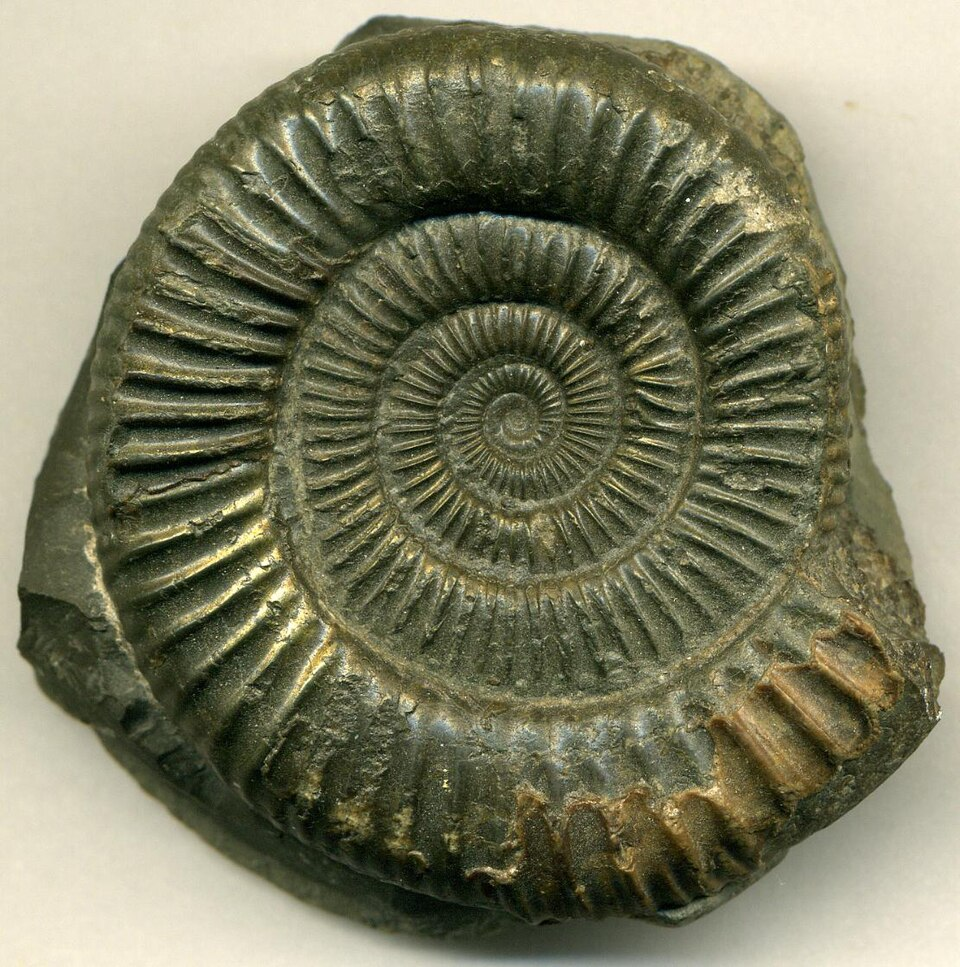
\includegraphics[height=4.6cm]{images/book1/g7-ammonite.jpg}

{\small An ammonite, an extinct animal with a coiled shell, a relative
of the squids and octopuses, \qty{5.7}{cm} across, from the \omterm{def:g1:landscapes-around-us:water}{coast} of
Yorkshire (England).}
\end{minipage}\hfill
\begin{minipage}[t]{0.49\linewidth}\centering
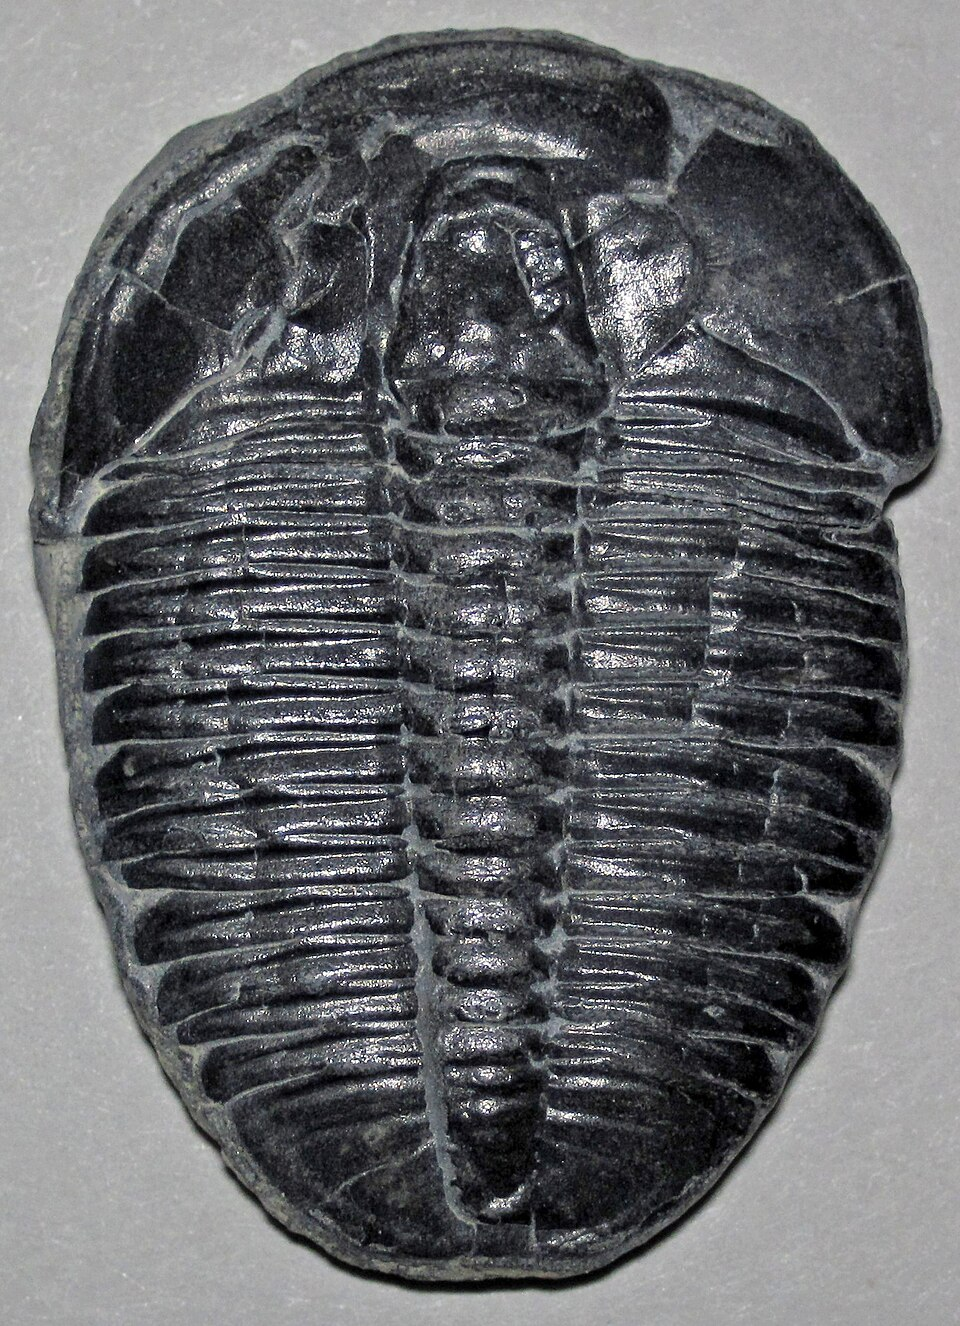
\includegraphics[height=4.6cm]{images/book1/g7-trilobite.jpg}

{\small A trilobite, an extinct \omterm{def:g2:water-on-earth:ocean}{sea} animal whose body has three lobes,
about \qty{2.6}{cm} across, from Utah (United States).}
\end{minipage}\par\medskip

{\small Two \omterm{def:g7:sediments-and-fossils:fossil}{fossils} of animals with hard shells. Photographs: James
St.~John (CC BY 2.0, via Wikimedia Commons).}
% ledger: commons:ammonite, commons:trilobite, nps:ammonoid, nps:trilobite
\label{fig:g7:sediments-and-fossils:ammonite-trilobite}
\end{omfigure}

Sometimes the shell itself does not last. Buried in \omterm{def:g3:stones-pebbles-sand:sand}{sand}, it is slowly
dissolved by the water seeping through the grains, and only a hollow
remains, with the shape of the shell printed on its walls: a \omterm{def:g7:sediments-and-fossils:fossil}{mould}. If
\omterm{def:g6:rocks-and-minerals:mineral}{minerals} later settle in the hollow and fill it, they make a copy of the
shell: a \omterm{def:g7:sediments-and-fossils:fossil}{cast}.
% ledger: ucmp:casts-molds

\begin{omfigure}
\begin{tikzpicture}[font=\small, x=1cm, y=1cm,
    clam/.style={line width=0.5pt}]
  \foreach \p/\fillc/\title in {0/{omLithSand!50!white}/{a shell buried\\[-2pt]in sand}, 1/{white}/{the shell has dissolved:\\[-2pt]a mould}, 2/{black!40}/{minerals fill the mould:\\[-2pt]a cast}} {
    \begin{scope}[xshift=\p*4.9cm]
      \fill[omLithSand] (0,0) rectangle (4.2,2.6);
      \foreach \i in {0,...,40} {
        \pgfmathsetmacro{\gx}{0.1+mod(\i*0.53,4.0)}
        \pgfmathsetmacro{\gy}{0.1+mod(\i*0.37,2.4)}
        \fill[brown!60!black] (\gx,\gy) circle (0.025);
      }
      \fill[\fillc, draw=brown!40!black, clam] (0.9,0.9) arc[start angle=180, end angle=0, x radius=1.2, y radius=0.95] -- cycle;
      \ifnum\p=1
        \foreach \a in {25,45,...,155} \draw[brown!50!black, line width=0.4pt] (2.1,0.9) -- ++(\a:0.93 and 0.75);
      \else
        \foreach \a in {25,45,...,155} \draw[brown!40!black, line width=0.4pt] (2.1,0.9) -- ++(\a:1.05 and 0.85);
      \fi
      \draw[black!70, line width=0.5pt] (0,0) rectangle (4.2,2.6);
      \node[anchor=north, align=center] at (2.1,-0.1) {\title};
    \end{scope}
  }
  \draw[-{Stealth[length=2.5mm]}, line width=1pt] (4.3,1.3) -- (4.8,1.3);
  \draw[-{Stealth[length=2.5mm]}, line width=1pt] (9.2,1.3) -- (9.7,1.3);
\end{tikzpicture}

{\small A \omterm{def:g7:sediments-and-fossils:fossil}{mould} and a \omterm{def:g7:sediments-and-fossils:fossil}{cast} (a drawing, cut through the \omterm{def:g3:stones-pebbles-sand:rock}{rock}). The
\omterm{def:g7:sediments-and-fossils:fossil}{mould} is the hollow, with the ribs of the shell printed on its wall; the
\omterm{def:g7:sediments-and-fossils:fossil}{cast} is a stone copy of the shell, made of the \omterm{def:g6:rocks-and-minerals:mineral}{minerals} that filled it.}
% ledger: ucmp:casts-molds
\label{fig:g7:sediments-and-fossils:mould-cast}
\end{omfigure}

Animals also leave \omterm{def:g7:sediments-and-fossils:fossil}{fossils} of what they did. An animal walking on the
soft, wet \omterm{def:g3:stones-pebbles-sand:sand}{mud} of a \omterm{def:g1:landscapes-around-us:water}{river} bank or a shore leaves footprints. Most are
washed away by the next wave or the next \omterm{def:g5:water-shapes-the-land:flood}{flood}. But if \omterm{def:g3:stones-pebbles-sand:sand}{sand} covers them
before they are erased, the footprint is filled, the \omterm{def:g3:stones-pebbles-sand:sand}{sand} later turns to
sandstone, and when the \omterm{def:g3:stones-pebbles-sand:rock}{rock} splits along the layer, it shows the
footprint and, on the other side, its \omterm{def:g7:sediments-and-fossils:fossil}{cast}.
% ledger: ucmp:footprints

\begin{omfigure}
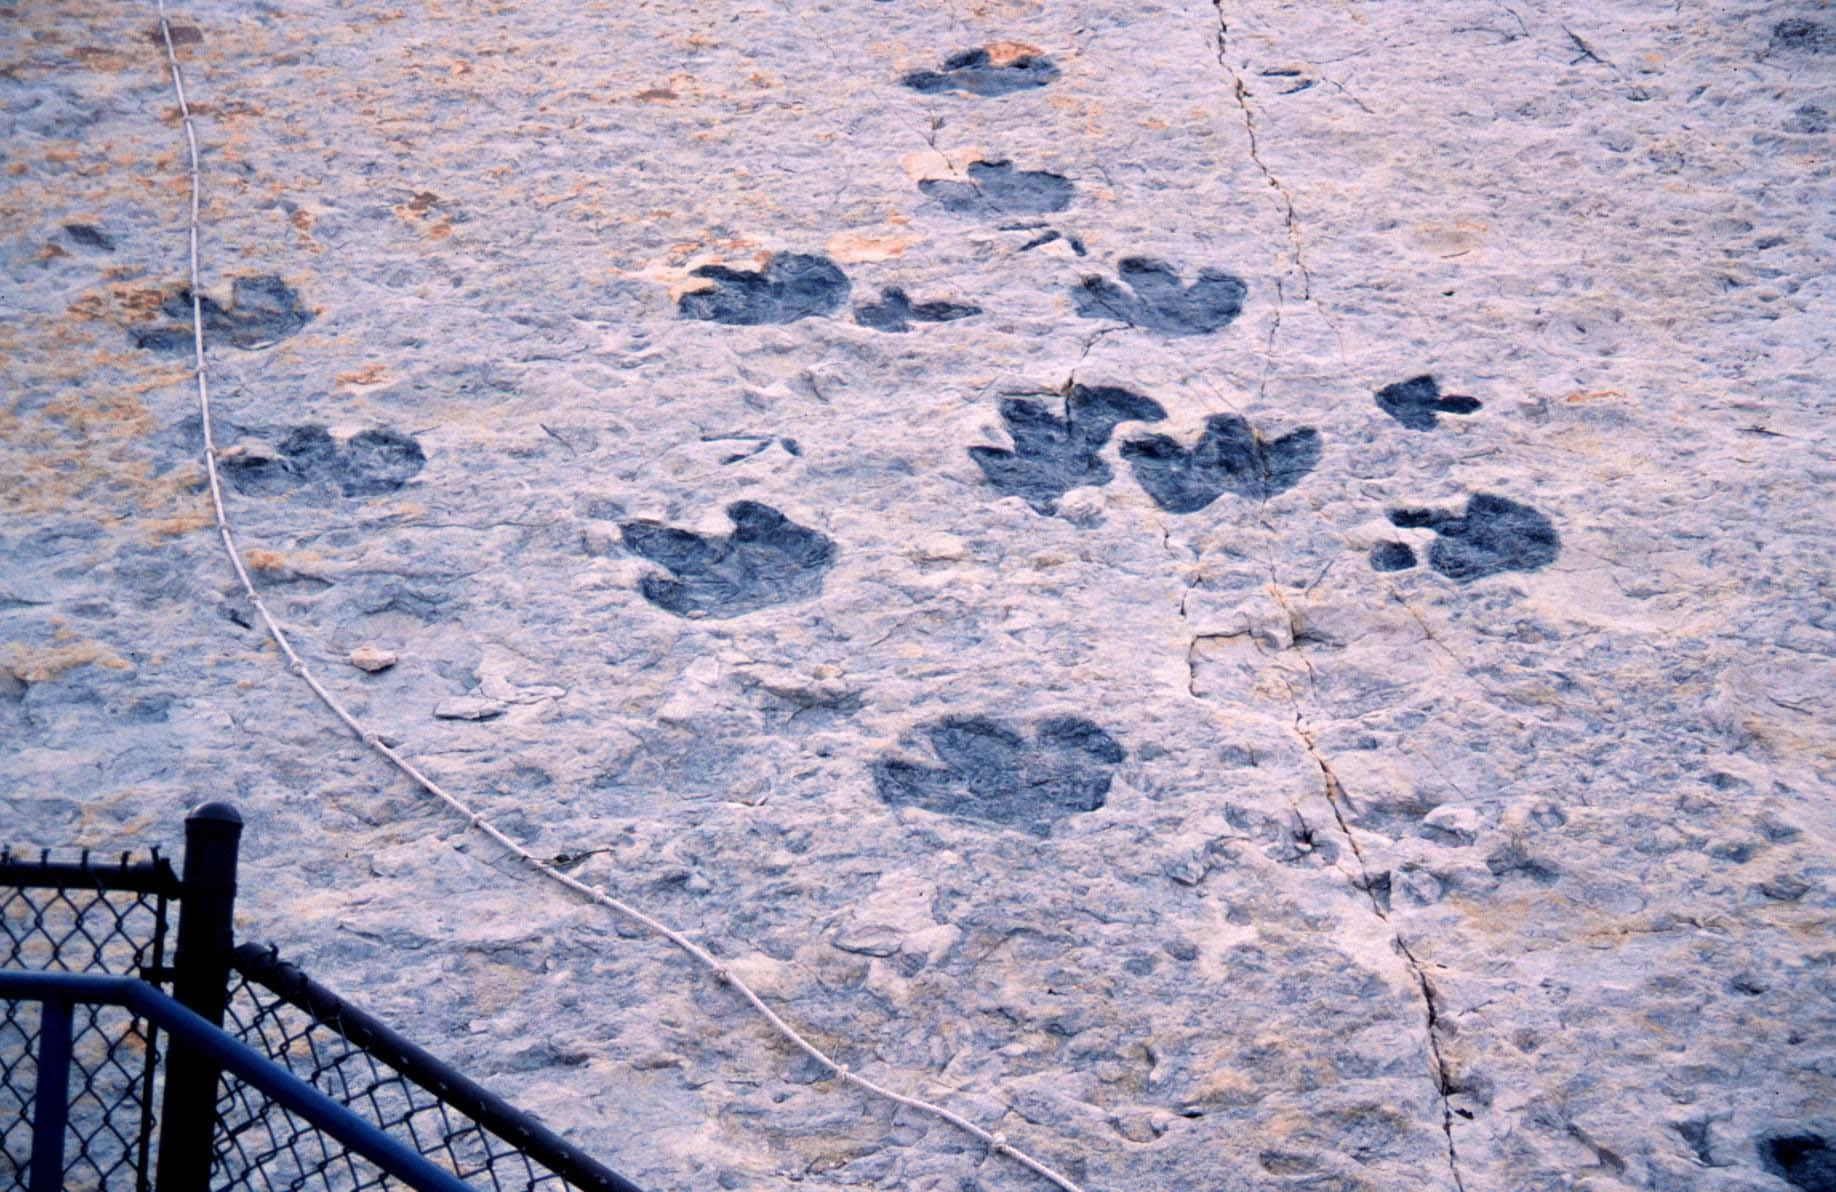
\includegraphics[width=0.62\linewidth]{images/book1/g7-dinosaur-tracks.jpg}

{\small Dinosaur footprints at Dinosaur Ridge, near Morrison, Colorado
(United States): dozens of tracks left in soft ground, now a tilted
surface of \omterm{def:g3:stones-pebbles-sand:rock}{rock}. Most were made by plant-eating dinosaurs, a few by
meat-eaters with slender toes. Photograph: Dexter Perkins (CC0, via
Wikimedia Commons).}
% ledger: commons:dino-tracks
\label{fig:g7:sediments-and-fossils:tracks}
\end{omfigure}

Biology uses \omterm{def:g7:sediments-and-fossils:fossil}{fossils} to follow the long history of living things. In
this book, \omterm{def:g7:sediments-and-fossils:fossil}{fossils} are clues of another kind: they tell us what the
place was like when the animal lived there.

\section{Layers and fossils, a record of the past}

Each layer keeps the marks of the place where it was laid down. Reefs of
coral grow today in warm, clear, shallow \omterm{def:g2:water-on-earth:ocean}{seas}; ripple marks form on \omterm{def:g3:stones-pebbles-sand:sand}{sand}
in shallow water, at the edge of a \omterm{def:g1:landscapes-around-us:water}{lake}, a \omterm{def:g1:landscapes-around-us:water}{river} or a \omterm{def:g2:water-on-earth:ocean}{sea}; coal formed
from the plants of ancient forests and marshes; brachiopods, crinoids
and trilobites lived only in the \omterm{def:g2:water-on-earth:ocean}{sea}. When the same clues are found in an old layer, the place
was probably like that when the layer formed.
% ledger: noaa:coral-where, nps:ripple-marks, nps:ripples-shallow, usgs:coal-origin, nps:trilobite

\begin{center}
\small
\begin{tabular}{|p{0.36\linewidth}|p{0.52\linewidth}|}
\hline
\textbf{clue in the layer} & \textbf{the place when the layer formed} \\
\hline
corals & a warm, shallow, clear \omterm{def:g2:water-on-earth:ocean}{sea} \\
\hline
shells of \omterm{def:g2:water-on-earth:ocean}{sea} animals (brachiopods, crinoids, trilobites) & a \omterm{def:g2:water-on-earth:ocean}{sea} \\
\hline
ripple marks on the surface of a layer & shallow water, at the edge of a \omterm{def:g1:landscapes-around-us:water}{lake}, a \omterm{def:g1:landscapes-around-us:water}{river} or a \omterm{def:g2:water-on-earth:ocean}{sea} \\
\hline
footprints & soft, wet \omterm{def:g3:stones-pebbles-sand:sand}{mud} or \omterm{def:g3:stones-pebbles-sand:sand}{sand}, often on a shore or a \omterm{def:g1:landscapes-around-us:water}{river} bank \\
\hline
coal & a swamp forest or a marsh \\
\hline
leaves and dragonfly wings & land, with plants growing \\
\hline
\end{tabular}
\end{center}
% ledger: noaa:coral-where, nps:grca-fossils, nps:trilobite, nps:ripple-marks, nps:ripples-shallow, ucmp:footprints, usgs:coal-origin

\begin{method}[Reading a layer]\label{met:g7:sediments-and-fossils:reading}
\begin{enumerate}
  \item Look at the grains: coarse grains settle where the water moves
        fast, fine \omterm{def:g3:stones-pebbles-sand:sand}{mud} only where it is calm.
  \item Look for \omterm{def:g7:sediments-and-fossils:fossil}{fossils} and marks (corals, shells, footprints, ripple
        marks, plant remains, coal) and use the table above.
  \item Put the clues together into one picture of the place: land or
        \omterm{def:g2:water-on-earth:ocean}{sea}, shallow or deep, calm or moving water.
\end{enumerate}
\end{method}

\begin{omfigure}
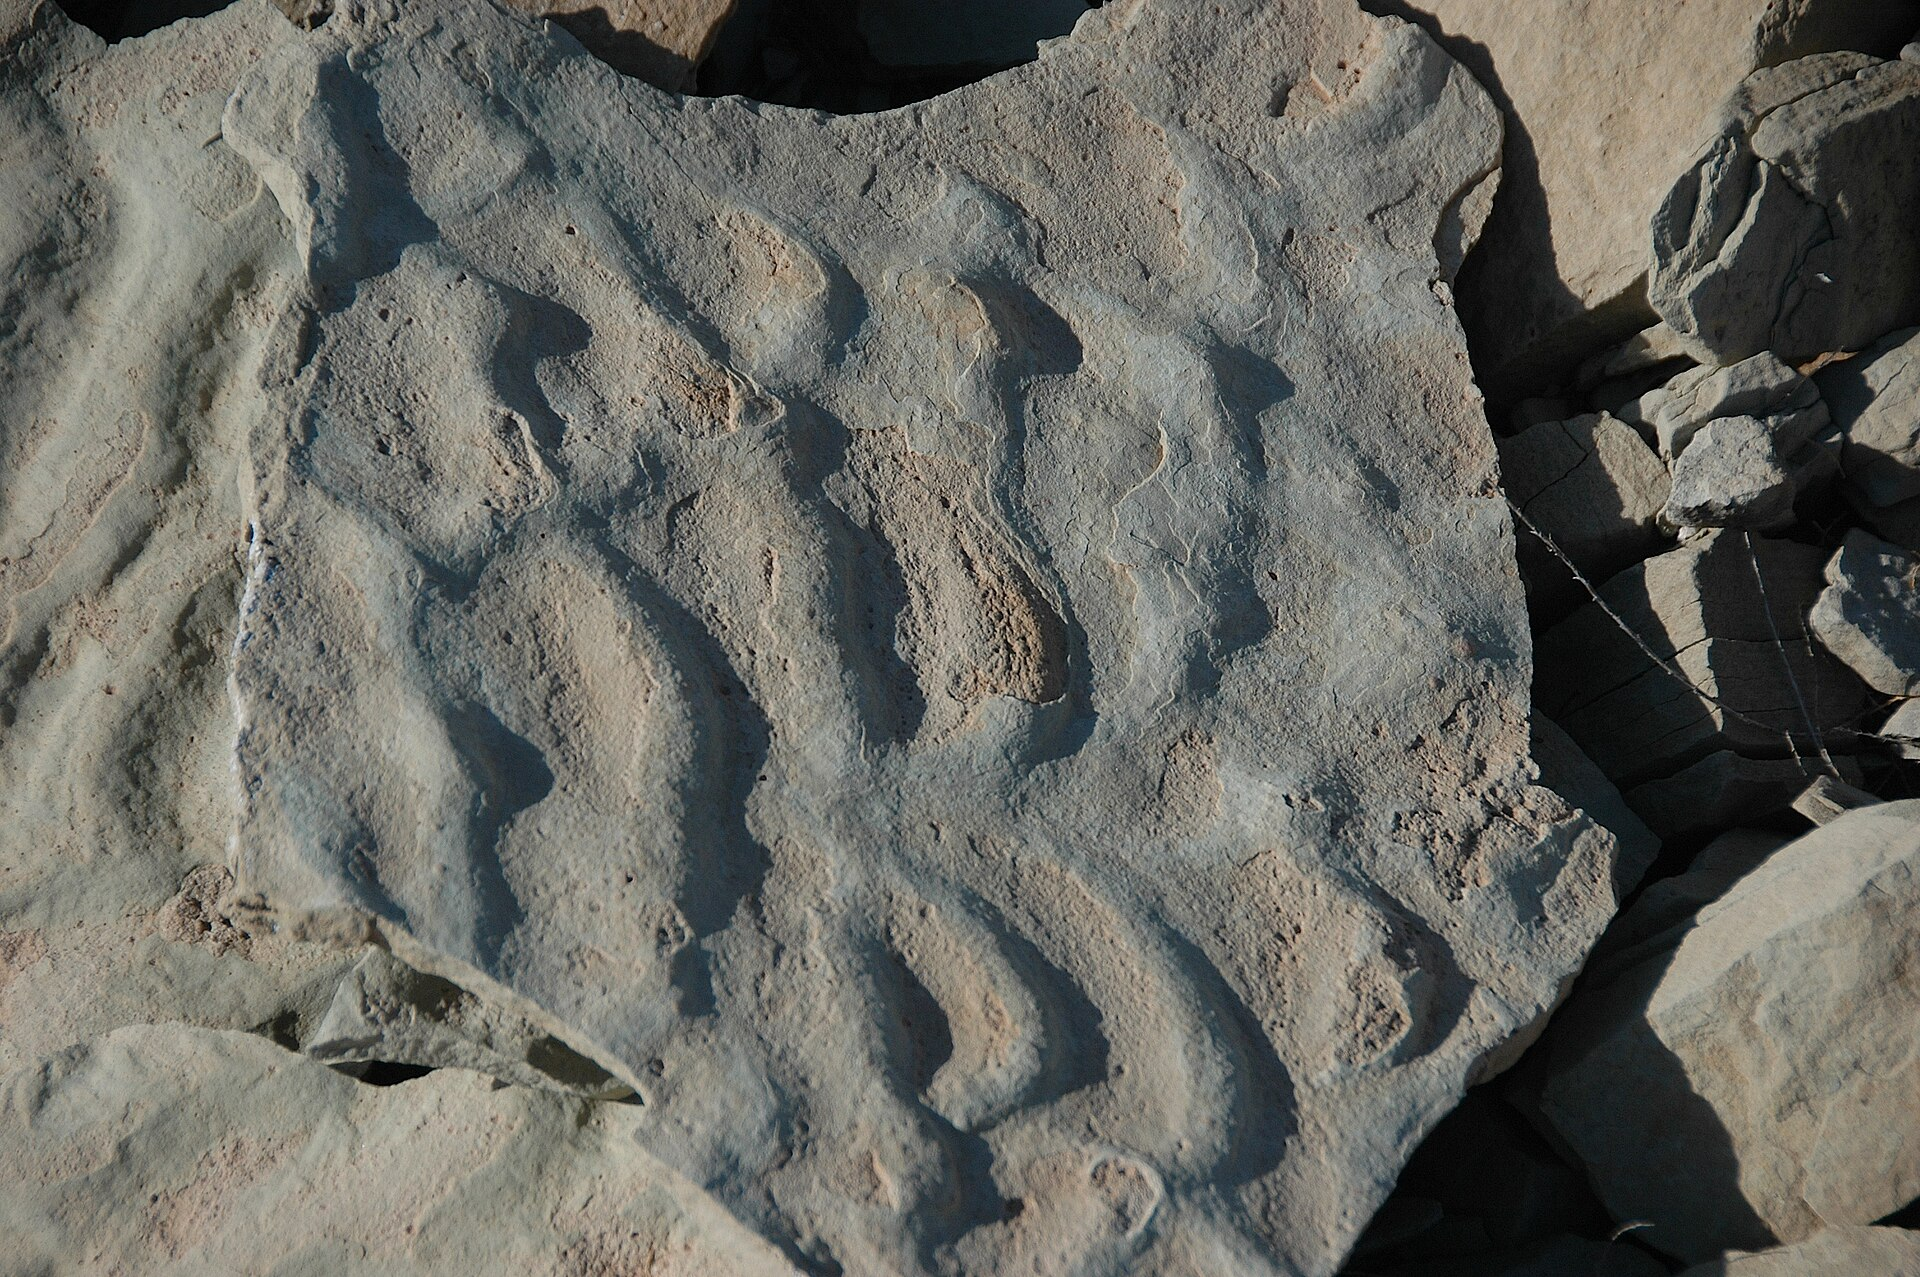
\includegraphics[width=0.56\linewidth]{images/book1/g7-ripple-marks.jpg}

{\small Ripple marks on a slab of sandstone in Capitol Reef National
Park, Utah (United States): the \omterm{def:g3:stones-pebbles-sand:sand}{sand} was once rippled by moving water,
like the \omterm{def:g3:stones-pebbles-sand:sand}{sand} of a beach or a stream bed today. Photograph: James
St.~John (CC BY 2.0, via Wikimedia Commons).}
% ledger: commons:ripples, nps:ripple-marks
\label{fig:g7:sediments-and-fossils:ripples}
\end{omfigure}

\begin{example}[The top of the Grand Canyon]\label{ex:g7:sediments-and-fossils:kaibab}
The Kaibab Limestone, the top layer of the Grand Canyon, is full of
brachiopod shells and the stem pieces of crinoids, both \omterm{def:g2:water-on-earth:ocean}{sea} animals. It
formed on the floor of a \omterm{def:g2:water-on-earth:ocean}{sea}. Today the same layer lies up to about
\qty{2700}{m} (\num{9000}~feet) above \omterm{def:g4:world-physical-map:altitude}{sea level}: since it formed, the
whole region has been raised.
% ledger: nps:grca-fossils, nps:grca-kaibab
\end{example}

A pile of layers can be drawn as a \emph{column}: the layers stacked in
the order they formed, with their thickness to scale and their clues
noted at the side. The column of the Varden Hills, the invented region
of the exercises of this series, is below.

\begin{omfigure}
\begin{tikzpicture}
  \begin{axis}[width=4.2cm, height=9.2cm, scale only axis=false, xmin=0, xmax=1, ymin=-60, ymax=485,
      axis x line=none, axis y line*=left, ytick={0,100,200,300,400},
      ylabel={metres above the base of the sandstone}, label style={font=\footnotesize},
      tick label style={font=\scriptsize}, clip=false]
    \addplot[lith schist, draw=black!70, line width=0.3pt] table {figdata/out/grade-7-varden_column-unit-older.dat};
    \addplot[lith sandstone, draw=black!70, line width=0.3pt] table {figdata/out/grade-7-varden_column-unit-sandstone.dat};
    \addplot[lith limestone, draw=black!70, line width=0.3pt] table {figdata/out/grade-7-varden_column-unit-limestone.dat};
    \addplot[lith shale, draw=black!70, line width=0.3pt] table {figdata/out/grade-7-varden_column-unit-shale.dat};
    \addplot[om lith={white}{om limestone}, draw=black!70, line width=0.3pt] table {figdata/out/grade-7-varden_column-unit-chalk.dat};
    \node[anchor=west, align=left, font=\footnotesize] at (axis cs:1.12,450) {\textbf{chalk}: its top has been\\worn away (only its base drawn)};
    \node[anchor=west, align=left, font=\footnotesize] at (axis cs:1.12,350) {\textbf{shale}, \qty{100}{m}: very fine grains;\\ammonites};
    \node[anchor=west, align=left, font=\footnotesize] at (axis cs:1.12,210) {\textbf{limestone}, \qty{180}{m}:\\corals and shells};
    \node[anchor=west, align=left, font=\footnotesize] at (axis cs:1.12,60) {\textbf{sandstone}, \qty{120}{m}:\\ripple marks, footprints};
    \node[anchor=west, align=left, font=\footnotesize] at (axis cs:1.12,-30) {older rocks (schist and granite),\\worn flat before the sandstone came};
  \end{axis}
\end{tikzpicture}

\medskip
{\small The column of the Varden Hills, the invented region of this
series: the layers in the order they formed, the first at the bottom,
with their thicknesses to scale. The \omterm{def:g7:sediments-and-fossils:fossil}{fossils} and marks noted at the side
are exercise data.}
% ledger: (invented region: figdata/shared/region.py, drawn by figdata/grade-7/varden_column.py)
\label{fig:g7:sediments-and-fossils:column}
\end{omfigure}

\begin{omfigure}
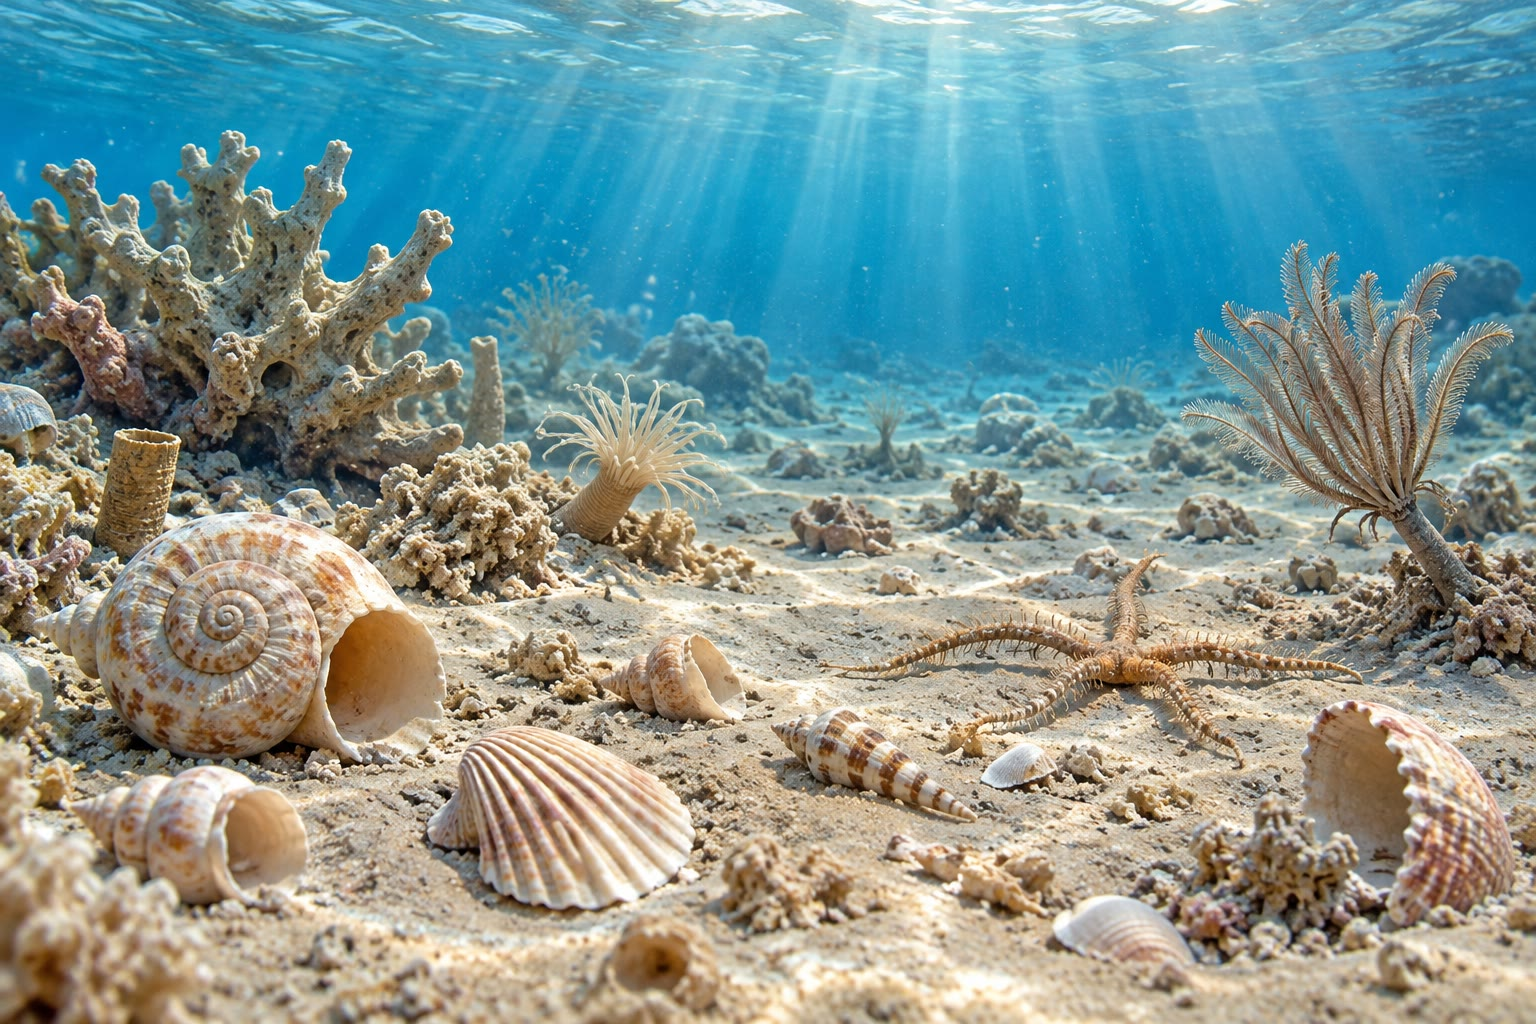
\includegraphics[width=0.6\linewidth]{images/book1/ai/g7-shallow-sea.jpg}

{\small A warm, shallow \omterm{def:g2:water-on-earth:ocean}{sea} floor of long ago, as it might have looked
while shells and coral pieces were settling into a future limestone
(AI-generated illustration of a generic scene).}
\label{fig:g7:sediments-and-fossils:shallow-sea}
\end{omfigure}

\begin{remark}[Look, photograph, leave it]\label{rem:g7:sediments-and-fossils:leave}
In many protected places, taking a \omterm{def:g7:sediments-and-fossils:fossil}{fossil} away is forbidden: in the Grand
Canyon, for example, it is against the law to dig up, move or take any
\omterm{def:g7:sediments-and-fossils:fossil}{fossil}. A visitor who finds one takes a photograph or makes a drawing,
leaves it where it is for others to see and for scientists to study,
and tells a ranger.
\end{remark}
% ledger: nps:grca-fossils

\begin{inthefield}[Sediments being laid down today]
On a beach, a \omterm{def:g1:landscapes-around-us:water}{lake} shore or the bank of a stream, with an adult, look at
the \omterm{def:g3:stones-pebbles-sand:sand}{sand} under shallow water: the moving water shapes it into ripples,
like the ones kept in the old sandstone. Leave a footprint in the wet
\omterm{def:g3:stones-pebbles-sand:sand}{sand} near the water's edge and watch what the next waves do to it. After
a rainy day, look at a puddle that has dried out: a thin skin of fine
\omterm{def:g3:stones-pebbles-sand:sand}{mud} often covers the \omterm{def:g3:stones-pebbles-sand:sand}{sand} at its bottom --- the finest grains settled
last, when the water was still. Draw what you see, and note where and
when.
\end{inthefield}
% ledger: nps:ripple-marks, ucmp:footprints, usgs:strata

\section{Exercises}

\begin{exercise}[$\star$]\label{exo:g7:sediments-and-fossils:1}
Match each word with its meaning: \omterm{def:g7:sediments-and-fossils:sediment}{sediment}; \omterm{def:g7:sediments-and-fossils:layer}{stratum}; \omterm{def:g7:sediments-and-fossils:fossil}{fossil}; \omterm{def:g7:sediments-and-fossils:fossil}{mould};
\omterm{def:g7:sediments-and-fossils:fossil}{cast}; \omterm{def:g7:sediments-and-fossils:fossil}{trace fossil}. (a) A hollow left in a \omterm{def:g3:stones-pebbles-sand:rock}{rock} where a shell has
dissolved. (b) A footprint or a burrow kept in a \omterm{def:g3:stones-pebbles-sand:rock}{rock}. (c) Loose material
laid down by water, wind or ice. (d) A stone copy made when a hollow
fills with \omterm{def:g6:rocks-and-minerals:mineral}{minerals}. (e) A sheet of \omterm{def:g7:sediments-and-fossils:sediment}{sediment} laid down at one time. (f)
The remains or trace of a living thing of long ago, kept in \omterm{def:g3:stones-pebbles-sand:rock}{rock}.
\end{exercise}

\begin{exercise}[$\star$]\label{exo:g7:sediments-and-fossils:2}
Put these steps in order, to tell how a shell becomes a \omterm{def:g7:sediments-and-fossils:fossil}{fossil} at the
surface: (a) \omterm{def:g5:water-shapes-the-land:erosion}{erosion} wears away the layers above it; (b) the animal dies
on the \omterm{def:g2:water-on-earth:ocean}{sea} floor; (c) new layers pile up and the shell turns to stone;
(d) \omterm{def:g3:stones-pebbles-sand:sand}{mud} covers the shell quickly.
\end{exercise}

\begin{exercise}[$\star$]\label{exo:g7:sediments-and-fossils:3}
Use the table of clues. Where did each layer form? (a) A limestone full
of corals. (b) A sandstone whose surface shows ripple marks. (c) A dark
layer of coal. (d) A shale with leaf prints and the wing of a dragonfly.
\end{exercise}

\begin{exercise}[$\star$]\label{exo:g7:sediments-and-fossils:4}
True or false? Correct the false ones. (a) Every animal that dies
becomes a \omterm{def:g7:sediments-and-fossils:fossil}{fossil} one day. (b) A footprint can be a \omterm{def:g7:sediments-and-fossils:fossil}{fossil}. (c) When muddy
water slows down, the fine \omterm{def:g3:stones-pebbles-sand:sand}{mud} settles first. (d) \omterm{def:g7:sediments-and-fossils:sediment}{Sediments} are laid
down flat.
\end{exercise}

\begin{exercise}[$\star\star$]\label{exo:g7:sediments-and-fossils:5}
Use the column of the Varden Hills. (a) Give the thickness of the
sandstone, the limestone and the shale. (b) What is their total
thickness? (c) What percentage of this total is limestone? Round to the
nearest whole number. (d) Why does the column give no thickness for the
chalk?
\end{exercise}

\begin{exercise}[$\star\star$]\label{exo:g7:sediments-and-fossils:6}
A pupil shakes a jar of water with \omterm{def:g3:stones-pebbles-sand:pebble}{gravel}, \omterm{def:g3:stones-pebbles-sand:sand}{sand} and \omterm{def:g3:stones-pebbles-sand:sand}{mud}, and lets it
settle. (a) Draw the jar the next day, and label the layers. (b) Why is
the water still cloudy after one hour? (c) She adds \omterm{def:g3:stones-pebbles-sand:sand}{sand} and \omterm{def:g3:stones-pebbles-sand:sand}{mud} again
and lets it settle. What does she see at the bottom now? (d) Which layer
of the jar formed first?
\end{exercise}

\begin{exercise}[$\star\star$]\label{exo:g7:sediments-and-fossils:7}
Which of these has the best chance of becoming a \omterm{def:g7:sediments-and-fossils:fossil}{fossil}, and which the
least? Explain. (a) A jellyfish washed onto a rocky shore. (b) A snail
shell buried in the \omterm{def:g3:stones-pebbles-sand:sand}{mud} of a calm \omterm{def:g1:landscapes-around-us:water}{lake}. (c) A bone lying for years on a
dry \omterm{def:g1:landscapes-around-us:landform}{plain}. (d) A clam shell covered by \omterm{def:g3:stones-pebbles-sand:sand}{sand} in a \omterm{def:g1:landscapes-around-us:water}{river} \omterm{def:g5:water-shapes-the-land:flood}{flood}.
\end{exercise}

\begin{exercise}[$\star\star$]\label{exo:g7:sediments-and-fossils:8}
A shell is buried in \omterm{def:g3:stones-pebbles-sand:sand}{sand} that becomes sandstone. Water seeping through
the \omterm{def:g3:stones-pebbles-sand:rock}{rock} dissolves the shell completely. (a) What is left in the \omterm{def:g3:stones-pebbles-sand:rock}{rock}?
(b) Later, \omterm{def:g6:rocks-and-minerals:mineral}{minerals} fill this hollow. What forms? (c) Is the shell itself
still there? (d) Why are \omterm{def:g7:sediments-and-fossils:fossil}{moulds} and \omterm{def:g7:sediments-and-fossils:fossil}{casts} found more often in sandstone
than in shale? (Think about how easily water passes between the grains.)
\end{exercise}

\begin{exercise}[$\star\star$]\label{exo:g7:sediments-and-fossils:9}
The Grand Canyon is on average \qty{1.6}{km} deep. (a) Write this depth in
metres. (b) Suppose the canyon walls were made of layers \qty{80}{m}
thick each: how many layers would fit from the rim to the bottom? (c) A
layer of \qty{160}{m} is what percentage of the depth?
\end{exercise}

\begin{exercise}[$\star\star$]\label{exo:g7:sediments-and-fossils:10}
Dinosaur footprints are found in a sandstone. (a) Were the dinosaurs
walking on hard \omterm{def:g3:stones-pebbles-sand:rock}{rock}? Explain. (b) Why do most footprints left on a
muddy shore disappear? (c) What had to happen soon after the dinosaurs
passed for the footprints to be kept? (d) Is a footprint a body \omterm{def:g7:sediments-and-fossils:fossil}{fossil}
or a \omterm{def:g7:sediments-and-fossils:fossil}{trace fossil}?
\end{exercise}

\begin{exercise}[$\star\star\star$]\label{exo:g7:sediments-and-fossils:11}
In a \omterm{def:g1:landscapes-around-us:water}{lake}, every \omterm{def:g5:water-shapes-the-land:flood}{flood} leaves a layer of \omterm{def:g3:stones-pebbles-sand:sand}{sand} about \qty{2}{cm} thick,
and the calm weeks after it a layer of \omterm{def:g3:stones-pebbles-sand:sand}{mud} about \qty{5}{mm} thick
(exercise data). (a) How thick, in millimetres, is one pair of layers?
(b) A \omterm{def:g6:inside-the-earth:layers}{core} taken from the \omterm{def:g1:landscapes-around-us:water}{lake} bottom is \qty{1}{m} long and made only of
such pairs. How many \omterm{def:g5:water-shapes-the-land:flood}{floods} does it record? (c) Near the \omterm{def:g1:landscapes-around-us:water}{river} \omterm{def:g5:water-shapes-the-land:source-mouth}{mouth} the
\omterm{def:g3:stones-pebbles-sand:sand}{sand} layers are thicker, far out they are thinner. Explain why. (d) Why
is there more \omterm{def:g3:stones-pebbles-sand:sand}{mud} than \omterm{def:g3:stones-pebbles-sand:sand}{sand} far from the \omterm{def:g5:water-shapes-the-land:source-mouth}{mouth}?
\end{exercise}

\begin{exercise}[$\star\star\star$]\label{exo:g7:sediments-and-fossils:12}
The \omterm{def:g7:sediments-and-fossils:fossil}{fossils} found in \omterm{def:g3:stones-pebbles-sand:rock}{rocks} are mostly shells and tiny remains; \omterm{def:g7:sediments-and-fossils:fossil}{fossils}
of soft animals are rare, and dinosaurs are only a very small part of
all \omterm{def:g7:sediments-and-fossils:fossil}{fossils}. (a) Explain why shells are so common. (b) Explain why soft
animals are rare. (c) A scientist wants to know all the animals that
lived in an ancient \omterm{def:g2:water-on-earth:ocean}{sea}. Can the \omterm{def:g7:sediments-and-fossils:fossil}{fossils} give the full list? Explain.
\end{exercise}

\section{Problem: The column of the Varden Hills}

\begin{problem}[{Weekend problem --- the layers of the Varden Hills are
read one by one, their fossils tell where they formed, and the time
needed to pile up the limestone is worked out}]
\label{pb:g7:sediments-and-fossils:1}
% ledger: (invented region: figdata/shared/region.py; rates are exercise data, figdata/grade-7/varden_column.py part rates)
Use the column of the Varden Hills in this chapter. Its sandstone shows
ripple marks and footprints; its limestone holds corals and shells; its
shale is made of very fine grains, with ammonites; the chalk at the top
has been partly worn away.

\medskip
\noindent\textbf{Part I --- Reading the layers.}\par\nopagebreak
\begin{enumerate}[beginpenalty=10000]
  \item List the four layers, from the first one laid down to the last.
  \item Give the thickness of the sandstone, the limestone and the shale,
        and their total.
  \item What percentage of this total is limestone?
  \item Why can nobody say how thick the chalk was when it formed?
\end{enumerate}

\medskip
\noindent\textbf{Part II --- The fossils in them.}\par\nopagebreak
\begin{enumerate}[resume, beginpenalty=10000]
  \item Where did the sandstone form? Give two clues.
  \item Where did the limestone form? Give the clue.
  \item The shale is made of very fine grains. Was the water calm or
        moving when it was laid down? Explain.
  \item Tell the story of the place in three sentences, from the
        sandstone to the shale.
\end{enumerate}

\medskip
\noindent\textbf{Part III --- How long it took.}\par\nopagebreak
\begin{enumerate}[resume, beginpenalty=10000]
  \item Write the thickness of the limestone in centimetres.
  \item Suppose the sandstone piled up by \qty{1}{cm} every 20 years. How
        many years did its \qty{120}{m} take?
  \item Suppose the limestone piled up by \qty{1}{cm} every 100 years.
        How many years did \qty{1}{m} of limestone take?
  \item How many years did the \qty{180}{m} of limestone take? How many
        times longer is that than the sandstone?
\end{enumerate}
\end{problem}
